\section{Implementation Details}
\label{sec:implementation}
In the following section, some implementation details will be highlighted. An entity relationship diagram explains the core data foundation of this project in \autoref{sub:db}, which represents the \gls{SKB} as described in \autoref{sub:SKB}. Overall the development of the intelligent agent could be accomplished with general techniques and features (such as the \gls{MVC} architecture) provided by \gls{RoR}. However, the details of the components related to \glspl{EAF} (see \autoref{sub:eaf_algorithm}) and \glspl{AF} (see \autoref{sub:af_algorithm}) should be highlighted, as they are crucial for the successful implementation. The requirements for \gls{R}-scripts entered into the application will be presented in \autoref{sec:r_code}.
	

	%\todo{Program listings (depending on the project nature). Complete source code listings must be submitted as an appendix to the report (excluding any well-known, freely obtainable, third-party libraries explicitly mentioned in the report). In addition, the source code must be submitted in a compressed file via KEATS together with the report. You should try to help the reader to navigate through your source code by providing a "table of contents" (titles of these files/units and one line descriptions). The first page of the program listings folder must contain the following statement certifying the work as your own: "I verify that I am the sole author of the programs contained in this folder, except where explicitly stated to the contrary". Your (typed) signature and the date should follow this statement.}

\subsection{Entity Relationship Class Diagram }
\label{sub:db}


The underlying database structure of the developed application is mostly influenced by the \gls{SKB} and the representation of \texttt{Assumptions} as classes. \autoref{fig:er} shows an overview over most of the involved database models used in this application. Additional classes like \texttt{Users}, \texttt{Abilities}, etc. are intentionally left out as this would add an additional level of complexity. 

\begin{figure}[!h]
	\centering
	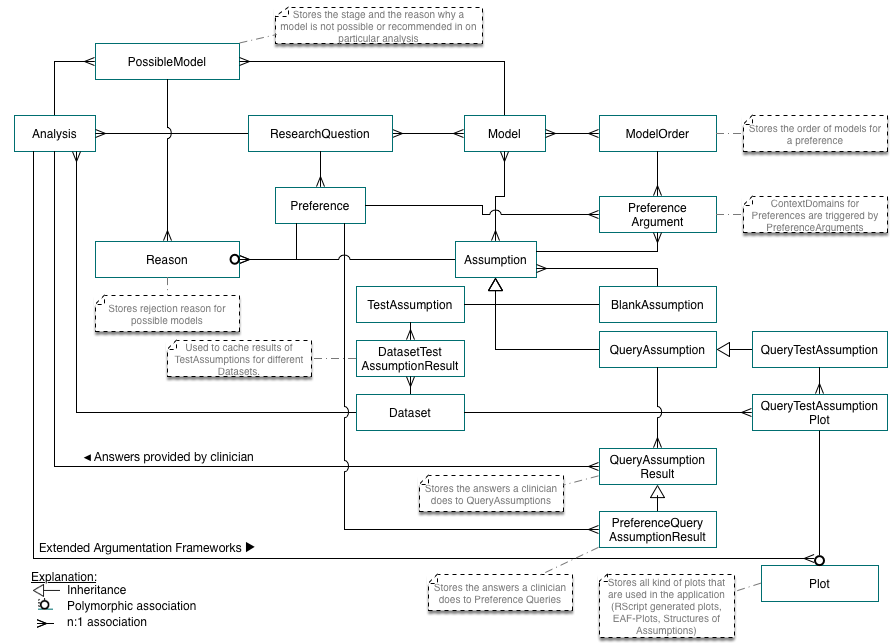
\includegraphics[width=\textwidth]{figures/er_complete}
	\caption{Entity-Relationship Diagram of the major classes used int the application. }
	\label{fig:er}
\end{figure}


The most important class is the \texttt{Analysis} which is associated with a \texttt{Dataset}, a \texttt{ResearchQuestion}, has many answered or open \texttt{QueryAssumptionResults} (this class stores the answers of a clinician to one particular \texttt{QueryAssumption}), and a list of \texttt{PossibleModels} (including impossible models and there \texttt{Reason} why they got rejected). 

The \gls{SKB} is represented by \texttt{ResearchQuestions} that have and belong to many \texttt{Models}. Each of these has multiple \texttt{Assumptions} that need to hold for this \texttt{Model}. These \texttt{Assumptions} have different specialisations: 

\bigskip

\begin{itemize}

	\item \texttt{TestAssumption}: An assumption that requires a \texttt{R} script to be executed and to return \texttt{true} or \texttt{false}. These assumptions will be checked automatically from the system and rely only on the dataset used in an analysis.
	\item \texttt{QueryAssumption}: A clinician has to provide a \textit{yes} or \textit{no} answer to a question during the process of the analysis. Only if he answers positively, this assumption holds.
	\item \texttt{QueryTestAssumption}: A \texttt{R} script generates a plot based on the dataset, which is then presented to the user who has to confirm that the plot shows some required features.
	\item \texttt{BlankAssumption}: An assumption that represents a grouping ability for other assumptions. All assigned assumptions (regardless of their type) must hold. 
\end{itemize}
\bigskip


\texttt{Preferences} have different \texttt{PreferenceArguments} that represent a specific \gls{CD} which are assigned to a particular \texttt{ModelOrder}. This allows the representation of \glspl{CD}, their order and the expressed preferences as described in \autoref{sub:SKB} in a generic way without limiting the triggers for a \gls{CD} to any particular \texttt{Assumption} type. 

The class \texttt{DatasetTestAssumptionResult} stores for each \texttt{TestAssumption} and each \texttt{Dataset} a pre-calculated result to enhance the speed of the evaluation during new \texttt{Analses}. \texttt{PreferenceQueryAssumptionResults} and \texttt{QueryAssumptionResults} store the answers of clinicians to \texttt{(Test)QueryAssumptions} for one particular \texttt{Analysis}.


\subsection{Extended Argumentation Framework: Algorithm}
\label{sub:eaf_algorithm}

An algorithm to solve \glspl{EAF} was presented in \cite{Dunne10computationin} (see \cref{fig:eaf_algo}) and is used to solve acceptability w.r.t. a subset $S' \subseteq \X$ of an argument $x \in \X$ in an \gls{EAF}. The presented algorithm defines an \gls{EAF} as a triple $\langle \X, \A, \D \rangle$ (\autoref{sub:eaf} introduced it as $\langle \S, \R, \D \rangle$).
This algorithm transforms an \gls{EAF} into an \gls{AF} using a colouring-based approach. To do so, it eliminates the attack-on-attacks relation $\D$ by removing elements from $\A$ according to the provided subset $S'$. In addition, \cref{fig:af_algo} (see \cref{sub:af_algorithm}) will be applied to check whether $x$ is acceptable w.r.t. $S'$ in the resulting AF $\langle \X', \A' \rangle$\footnote{As the \gls{EAF} gets reduced to an \gls{AF} the following is true: $\X' \subseteq \X, \A' \subseteq \A$.}.


\begin{algorithm}[!htp]
	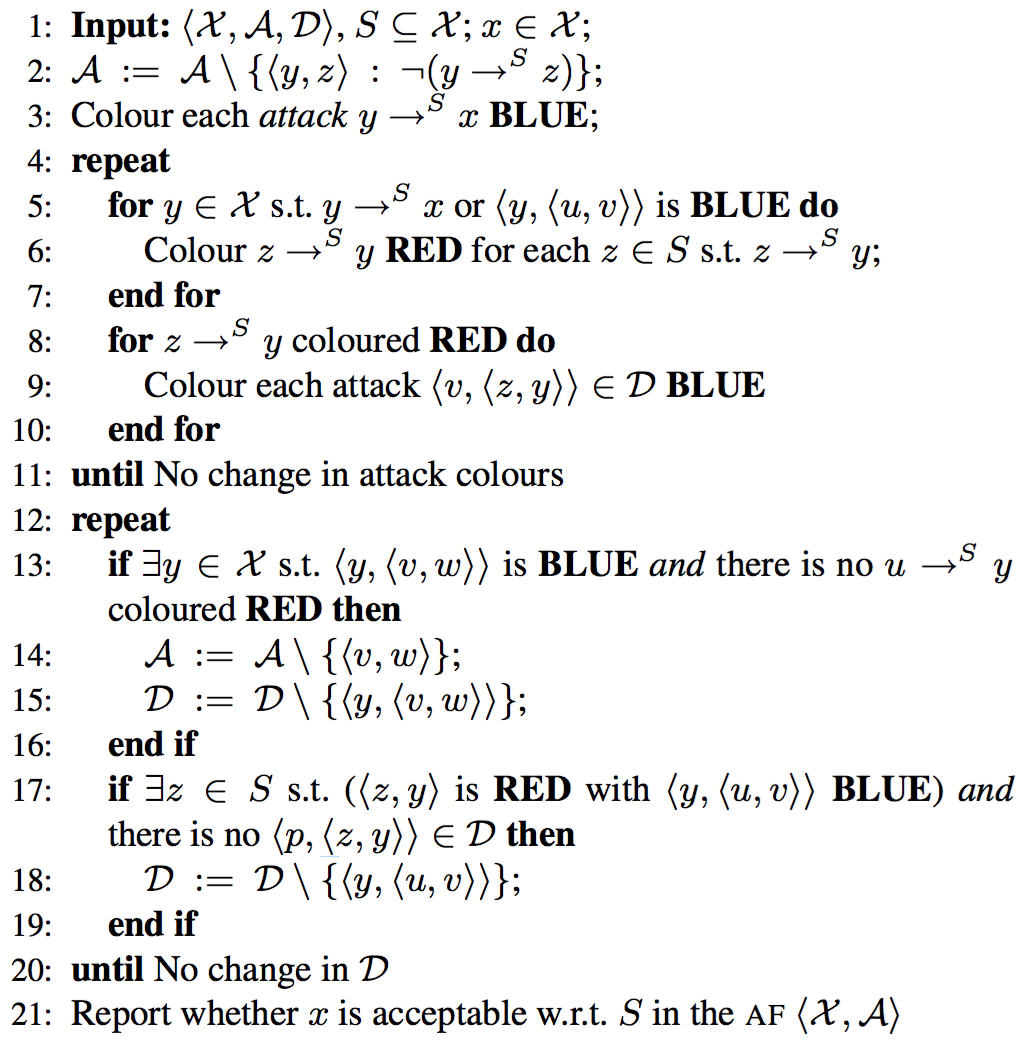
\includegraphics[width=0.8\textwidth]{figures/eaf_algorithm}
	\caption{Deciding \gls{EAF} Acceptability of $x \in \X$ w.r.t. $S' \subseteq \X$ in $\langle \X, \A, \D \rangle$.}
	\label{fig:eaf_algo}
\end{algorithm}


\subsection{Argumentation Framework: Algorithm}
\label{sub:af_algorithm}

The algorithm presented in \cref{fig:af_algo} is based on an labelling approach proposed in \cite{Modgil2009Proof, rodrigues}. It is supposed to calculate the preferred extensions of an \gls{AF}. \texttt{Cand} holds the possible candidates for a preferred labelling as defined in \cref{def:preferred_extension} and is initialised with \texttt{Cand = $\emptyset$}. The Ruby implementation of this algorithm can be found in \cref{lst:af}. The used class \texttt{Labeling} can be found in the provided source code. 

\begin{algorithm}[!htp]
	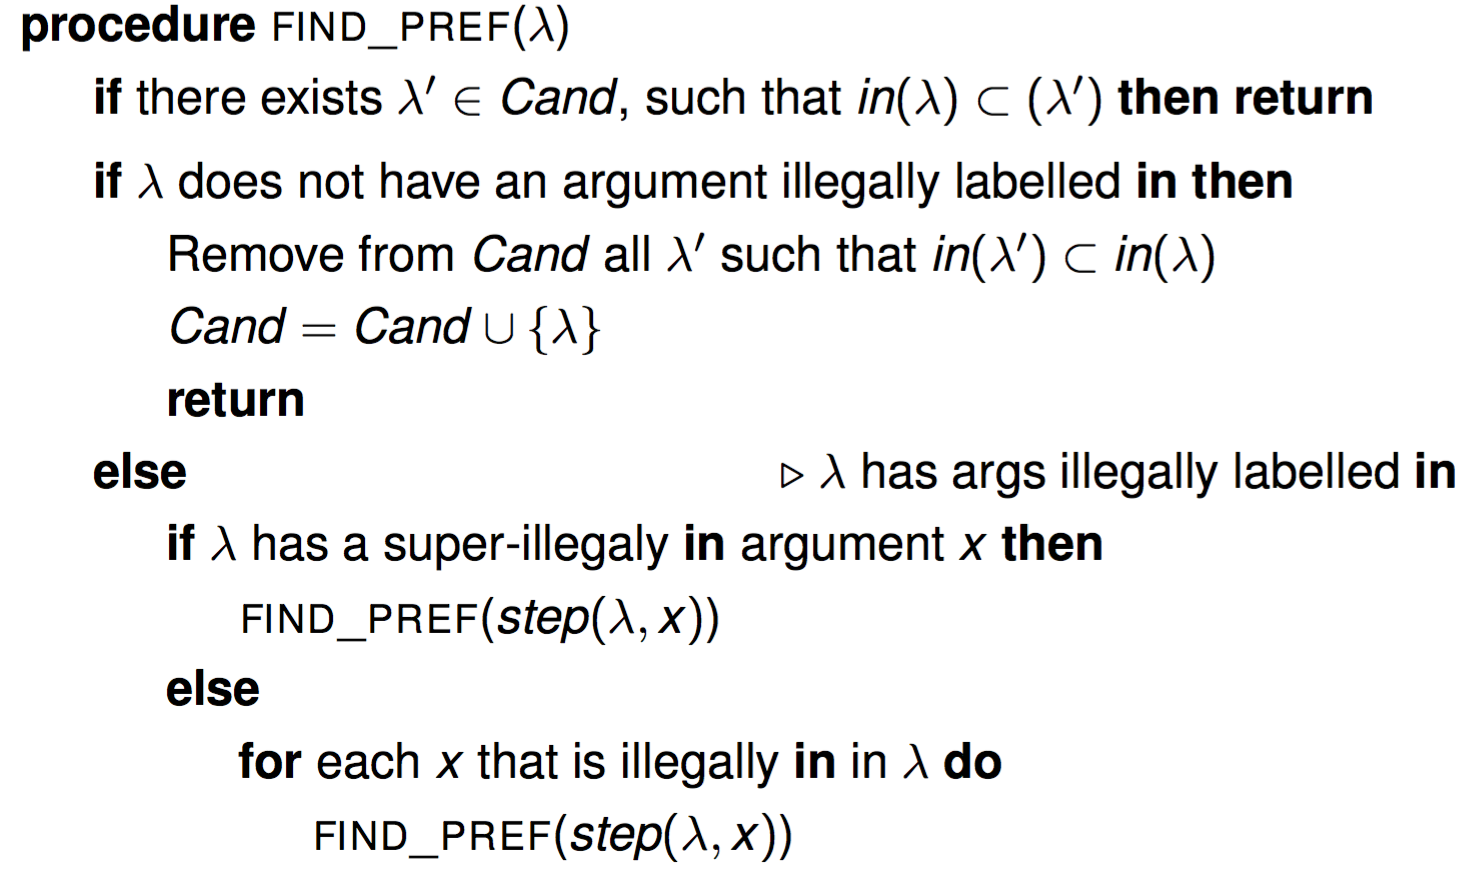
\includegraphics[width=0.8\textwidth]{figures/af_labelling}
	\caption{Algorithm to compute preferred labelings $\lambda \in $ \texttt{Cand} for \glspl{AF} \cite{rodrigues}.}
	\label{fig:af_algo}
\end{algorithm}



\subsection{R-Code and \texttt{rinruby} gem}
\label{sec:r_code}

To test if a \texttt{TestAssumption} holds or not, statisticians have to upload \gls{R}-scripts that verify these assumptions on the selected data set. This is done by executing the script in \gls{R} and returning the result back to the \gls{RoR} application. Therefore the scripts have to fulfil certain criteria to be able to communicate correctly with the rest of the agent. The provided scripts are executed using regular R-Syntax. In addition to the by default loaded libraries, the \texttt{survival} library will be installed on the executing systems, as it is often used during analyses related to statistical model selection.

Accessing the data setof the analysis as an input in the R-script is essential. The application supports only uploads of CSV files. Thereby the selected format of providing the data sets to the scripts was chosen to be a tabular representation as \gls{R} has an excellent support of loading CSV files.

\begin{listing}[htbp]
	\rcode{figures/mild_censoring.r}
	\caption{R-script to evaluate a \texttt{TestAssumption} on a data set to check whether the underlying data set has been mild censored or not. The performance measurement of CD1 relies on this check (see \autoref{tab:cd1}). }
	\label{lst:cd_mild}
\end{listing}


Each script that is executed will have access to the variable \texttt{tabular\_data} which has been initialised with \texttt{tabular\_data=read.csv(file='\#\{filename\}')}. This type of assumption must return its result (whether the assumption holds on this data set or not) in the boolean variable named \texttt{result}. The provided example in \cref{lst:cd_mild} shows, how this \texttt{tabular\_data} and the \texttt{result} variable are used together to perform an assumption check on the data set.

A \texttt{QueryTestAssumption} will receive the additional variable \texttt{fileName} which is initialised with an absolute filename to a temporary file. This must be used to store a generated plot during the analysis, as the hosted application does not have read and write access to all folders. For this type of assumption it is necessary to return a valid PNG at the provided file location. Please note, that due to some rendering issues, the Heroku hosted installation only supports PNG generation in R-scripts when the \texttt{type} is set to \texttt{cairo} (see \cref{lst:rcode}).

To execute the \gls{R}-scripts the gem \texttt{rinruby}\footnote{\url{https://github.com/clbustos/rinruby}} has been used. As the original gem did not provide all required functionalities and features it has been extended and forked at \href{https://github.com/sebastianzillessen/rinruby}{https://github.com/sebastianzillessen/rinruby}. 

In addition to this, separate so called buildpacks have been used to enable \gls{R}\footnote{\url{https://github.com/virtualstaticvoid/heroku-buildpack-r}} and the generation of plots\footnote{\url{https://github.com/weibeld/heroku-buildpack-graphviz.git}} on Heroku. 

